\pdfminorversion=4
\documentclass{beamer}
\usepackage[T1]{fontenc}
\usepackage[ngerman]{babel}
\usepackage[utf8]{inputenc}
\usepackage[babel,german=quotes]{csquotes}
\usepackage{amsmath,amsfonts,amssymb}
\usepackage{hyperref}
\usepackage{lmodern}
\usepackage{microtype}

\usetheme{fau-4-3}

\usepackage[sort&compress,comma,super,square]{natbib}
%\bibliographystyle{apalike} % Or your specific bibliographystyle
\bibliographystyle{unsrtdin}
%\bibliographystyle{gerplain}

\newcommand{\todo}[1]{\textbf{\color{red}{TODO: #1}}}


\title{cowbusconfig – Ansatz zur dezentralen Konfiguration von Gebäudeautomation}
\author[P. Kanzler, M. Zapf]{Patrick\,Kanzler \and Michael\,Zapf}
\institute{14. GI/ITG KuVS Fachgespraech \enquote{Sensornetze}, Erlangen}
\date{23.09.2015}

% space between items
\newcommand{\customitemsep}{7pt}
\newcommand{\customitemsepsub}{2pt}

\def\insertframetitle{}
\begin{document}
\frame{\titlepage}

%\section{cowbusconfig – Ansatz zur dezentralen Konfiguration von Gebaueudeautomation}
\begin{frame}
	\frametitle{Der Traum von der schönen neuen Welt}

	\begin{itemize} \setlength{\itemsep}{\customitemsep}
		\item \todo{schön darstellen, vielleicht mit Bildern, momentan nur Stichpunkte}
		\item das Haus der Zukunft, vernetzt und intelligent
		\item mögliche Anwendung: Beleuchtung verfolgt den Nutzer durch das Haus
        \item scheitert bisher: komplizierte Einrichtung, teure Komponenten, keine einheitlichen Standards
	\end{itemize}
\end{frame}

\begin{frame}
	\frametitle{Ansätze}
    \begin{columns}[c]
        \column[c]{10cm}
            \textbf{EIB/KNX} \cite{knx-prod}
            \begin{itemize} \setlength{\itemsep}{\customitemsep}
                \item etabliertes System
                \item viele Produkte auf dem Markt
                    \vspace*{0.5cm}
                \item \textcolor{red}{aufwändige (Neu-)Einrichtung}
            \end{itemize}
            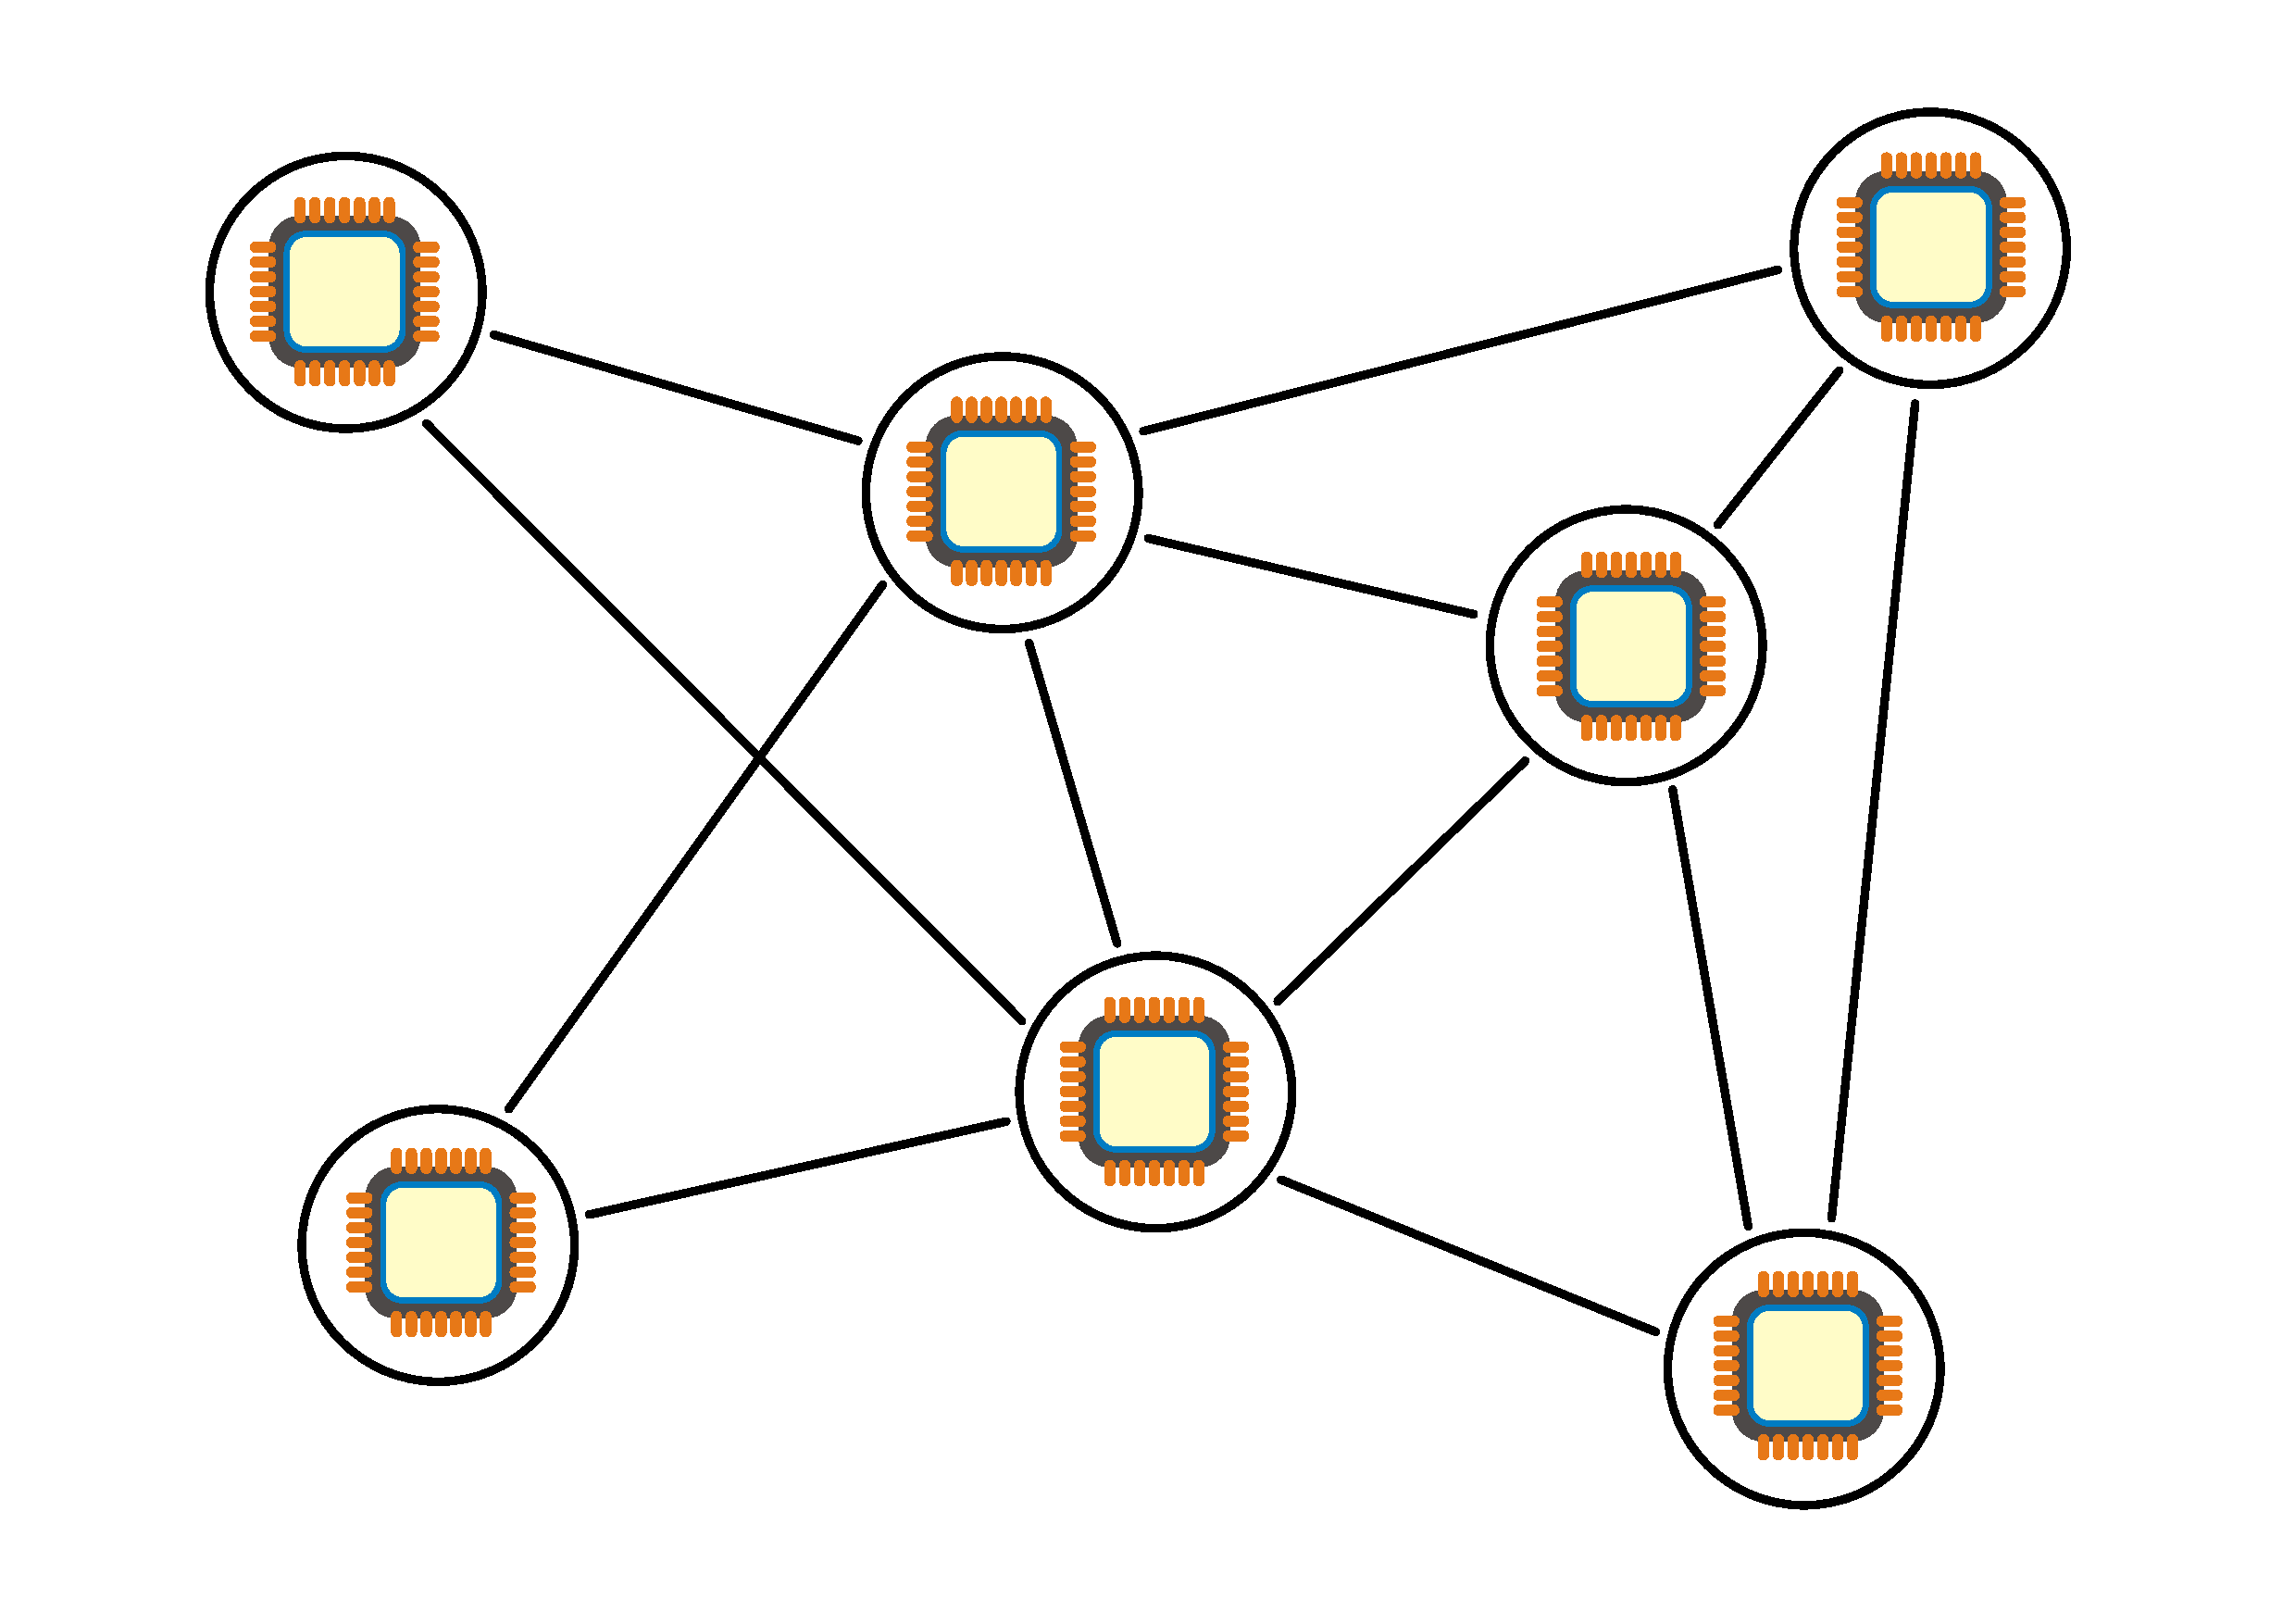
\includegraphics[width=.9\linewidth]{img/decentralize-network.pdf}
            \pause
        \column{10cm}
            \textbf{Skriptserver} \\
            {\fontsize{15pt}{18pt} \selectfont (z.\,B. nach Haenselmann et al. \cite{haenselmann2007skriptbasierte})}
            \begin{itemize} \setlength{\itemsep}{\customitemsep}
                \item zentrale Stelle mit Schaltregeln
                \item Skripte jederzeit anpassbar
                    \vspace*{0.5cm}
                \item \textcolor{red}{\enquote{Single Point of Failure}}
            \end{itemize}
            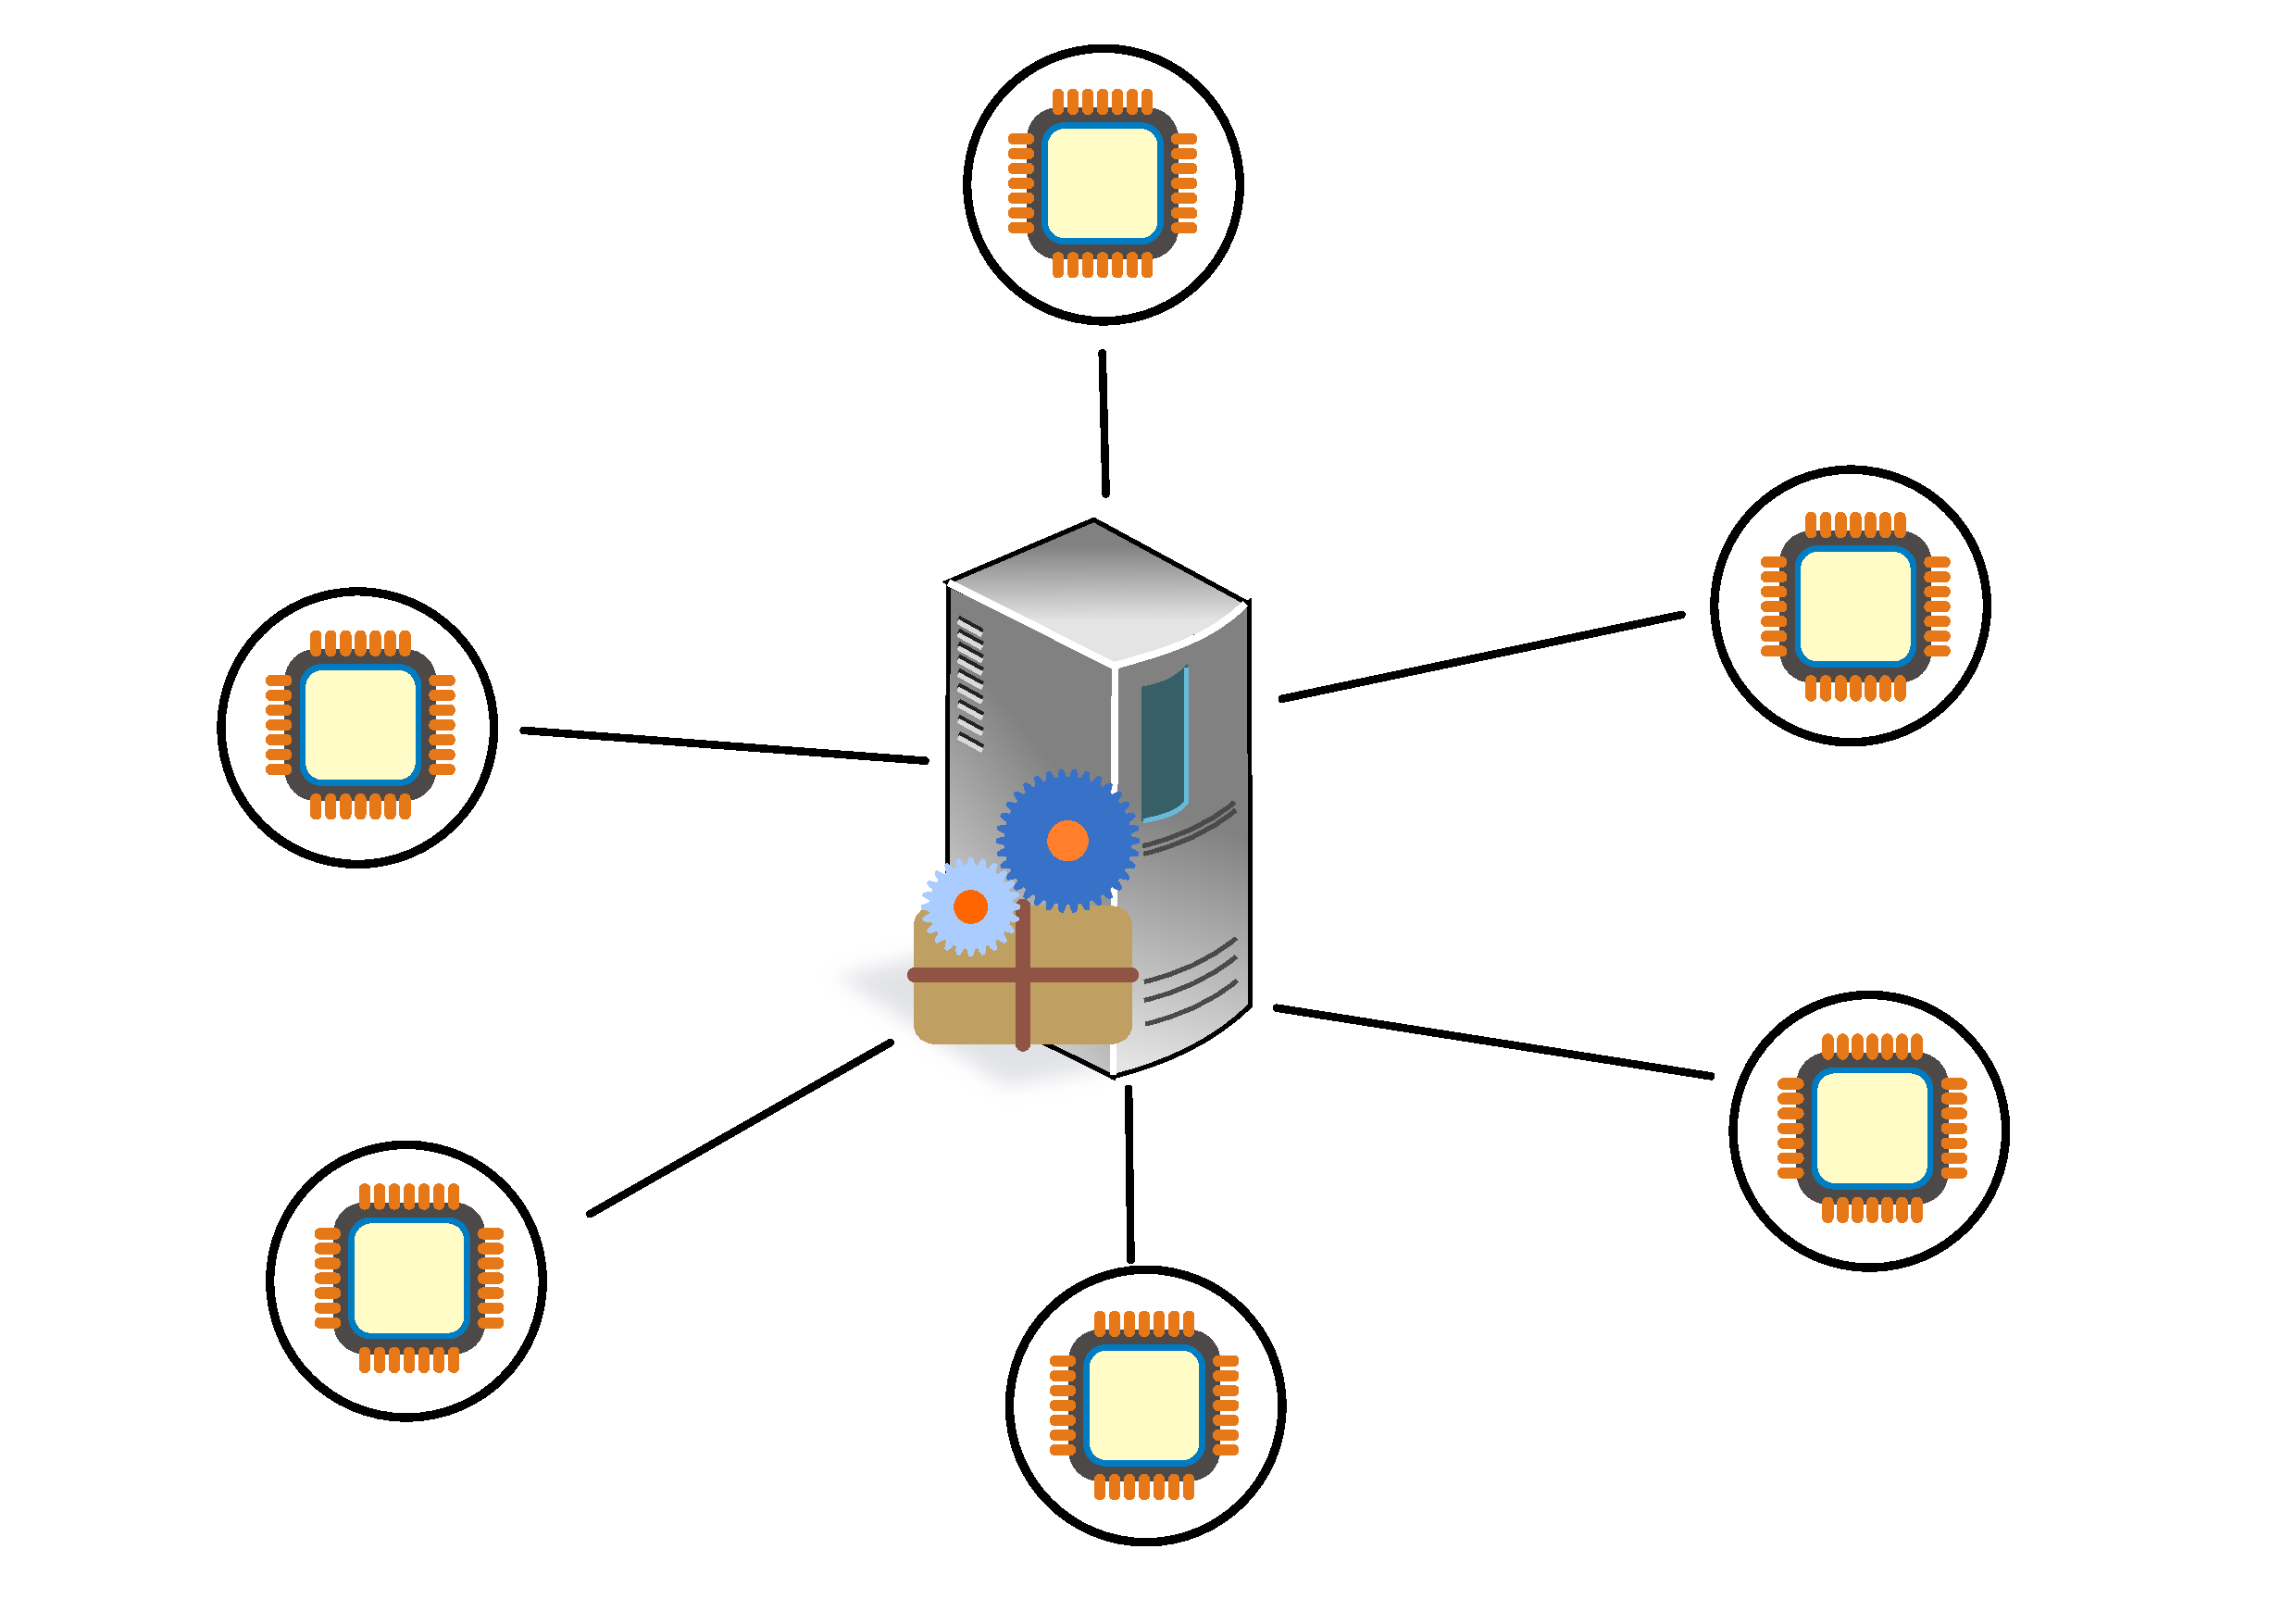
\includegraphics[width=.9\linewidth]{img/centralize-network.pdf}
    \end{columns}
\end{frame}

\begin{frame}
    \frametitle{Ziele und Ideen}

		    \begin{itemize} \setlength{\itemsep}{\customitemsep}
		        \item dezentrale Organisation
		        \item komfortable Konfiguration, nicht jeden Knoten \enquote{anfassen} müssen
		            \begin{itemize} \setlength{\itemsep}{\customitemsepsub}
		                \item z.\,B. Webbrowser vom Notebook/Tablet aus
		                \item[$\Rightarrow$] Gateway vom LAN/WLAN ins Sensornetz benötigt
		            \end{itemize}
		        
		        \pause
		        \item einfach nachvollziehbare Schaltregeln
		        \item typische Anforderungen an Energieversorgung beachten
		            \begin{itemize} \setlength{\itemsep}{\customitemsepsub}
		                \item oft: Aktoren besitzen stabile Stromversorgung
		                \item Sensoren eher klein, flexibel, sparsam
		                \item[$\Rightarrow$] Aufteilung in \enquote{dumme} Sensoren und \enquote{intelligente} Aktoren
		                \item[$\Rightarrow$] eigentliche Entscheidungs- bzw. Schaltlogik in Aktoren
		            \end{itemize}
		            
		    \end{itemize}
\end{frame}

\begin{frame}
    \frametitle{Regeln}

    \begin{itemize} \setlength{\itemsep}{\customitemsep}
        \item Annahmen: 
            \begin{itemize}
                \item (virtuelle) Knoten durch eindeutige Adresse identifizierbar
                \item Sensorpaket enthält nur einen Wert, Bedeutung bekannt
            \end{itemize}
        \item[ ] \vspace*{0.2cm}
            \pause
        \item Regel setzt sich zusammen aus:
        	\begin{itemize}
        		\item Quelladresse
		        \item Typ des Vergleichs ($<$, $>$, ==, !=, $<>$)
		        \item Grenzwert(e)
		        \item auszuführende Aktion
	            \begin{itemize} \setlength{\itemsep}{\customitemsep}
        	        \item Muss dem Aktor bekannt sein!
            	\end{itemize}
        	\end{itemize}
    \end{itemize}
\end{frame}

\begin{frame}
    \frametitle{Konfigurationsnachrichten}

        Ziele:
            \begin{itemize} \setlength{\itemsep}{\customitemsep}
                \item Kommunikation in-band, Standort egal
                \item Konfiguration jederzeit auslesbar und änderbar
            \end{itemize}

            \pause
        \vspace*{1cm}


        3 Typen ausreichend: LIST, ADD, DELETE
            \begin{itemize} \setlength{\itemsep}{\customitemsep}
                \item \textbf{LIST} fordert alle Regeln eines Knotens an
                \item \textbf{ADD} erstellt eine neue Regel auf einem Knoten
                \item \textbf{DELETE\_ONE} löscht eine Regel auf einem Knoten
            \end{itemize}
\end{frame}

\begin{frame}
    \frametitle{Demo}
		\begin{columns}
        	\column{.4\textwidth}
        	\uncover<1->{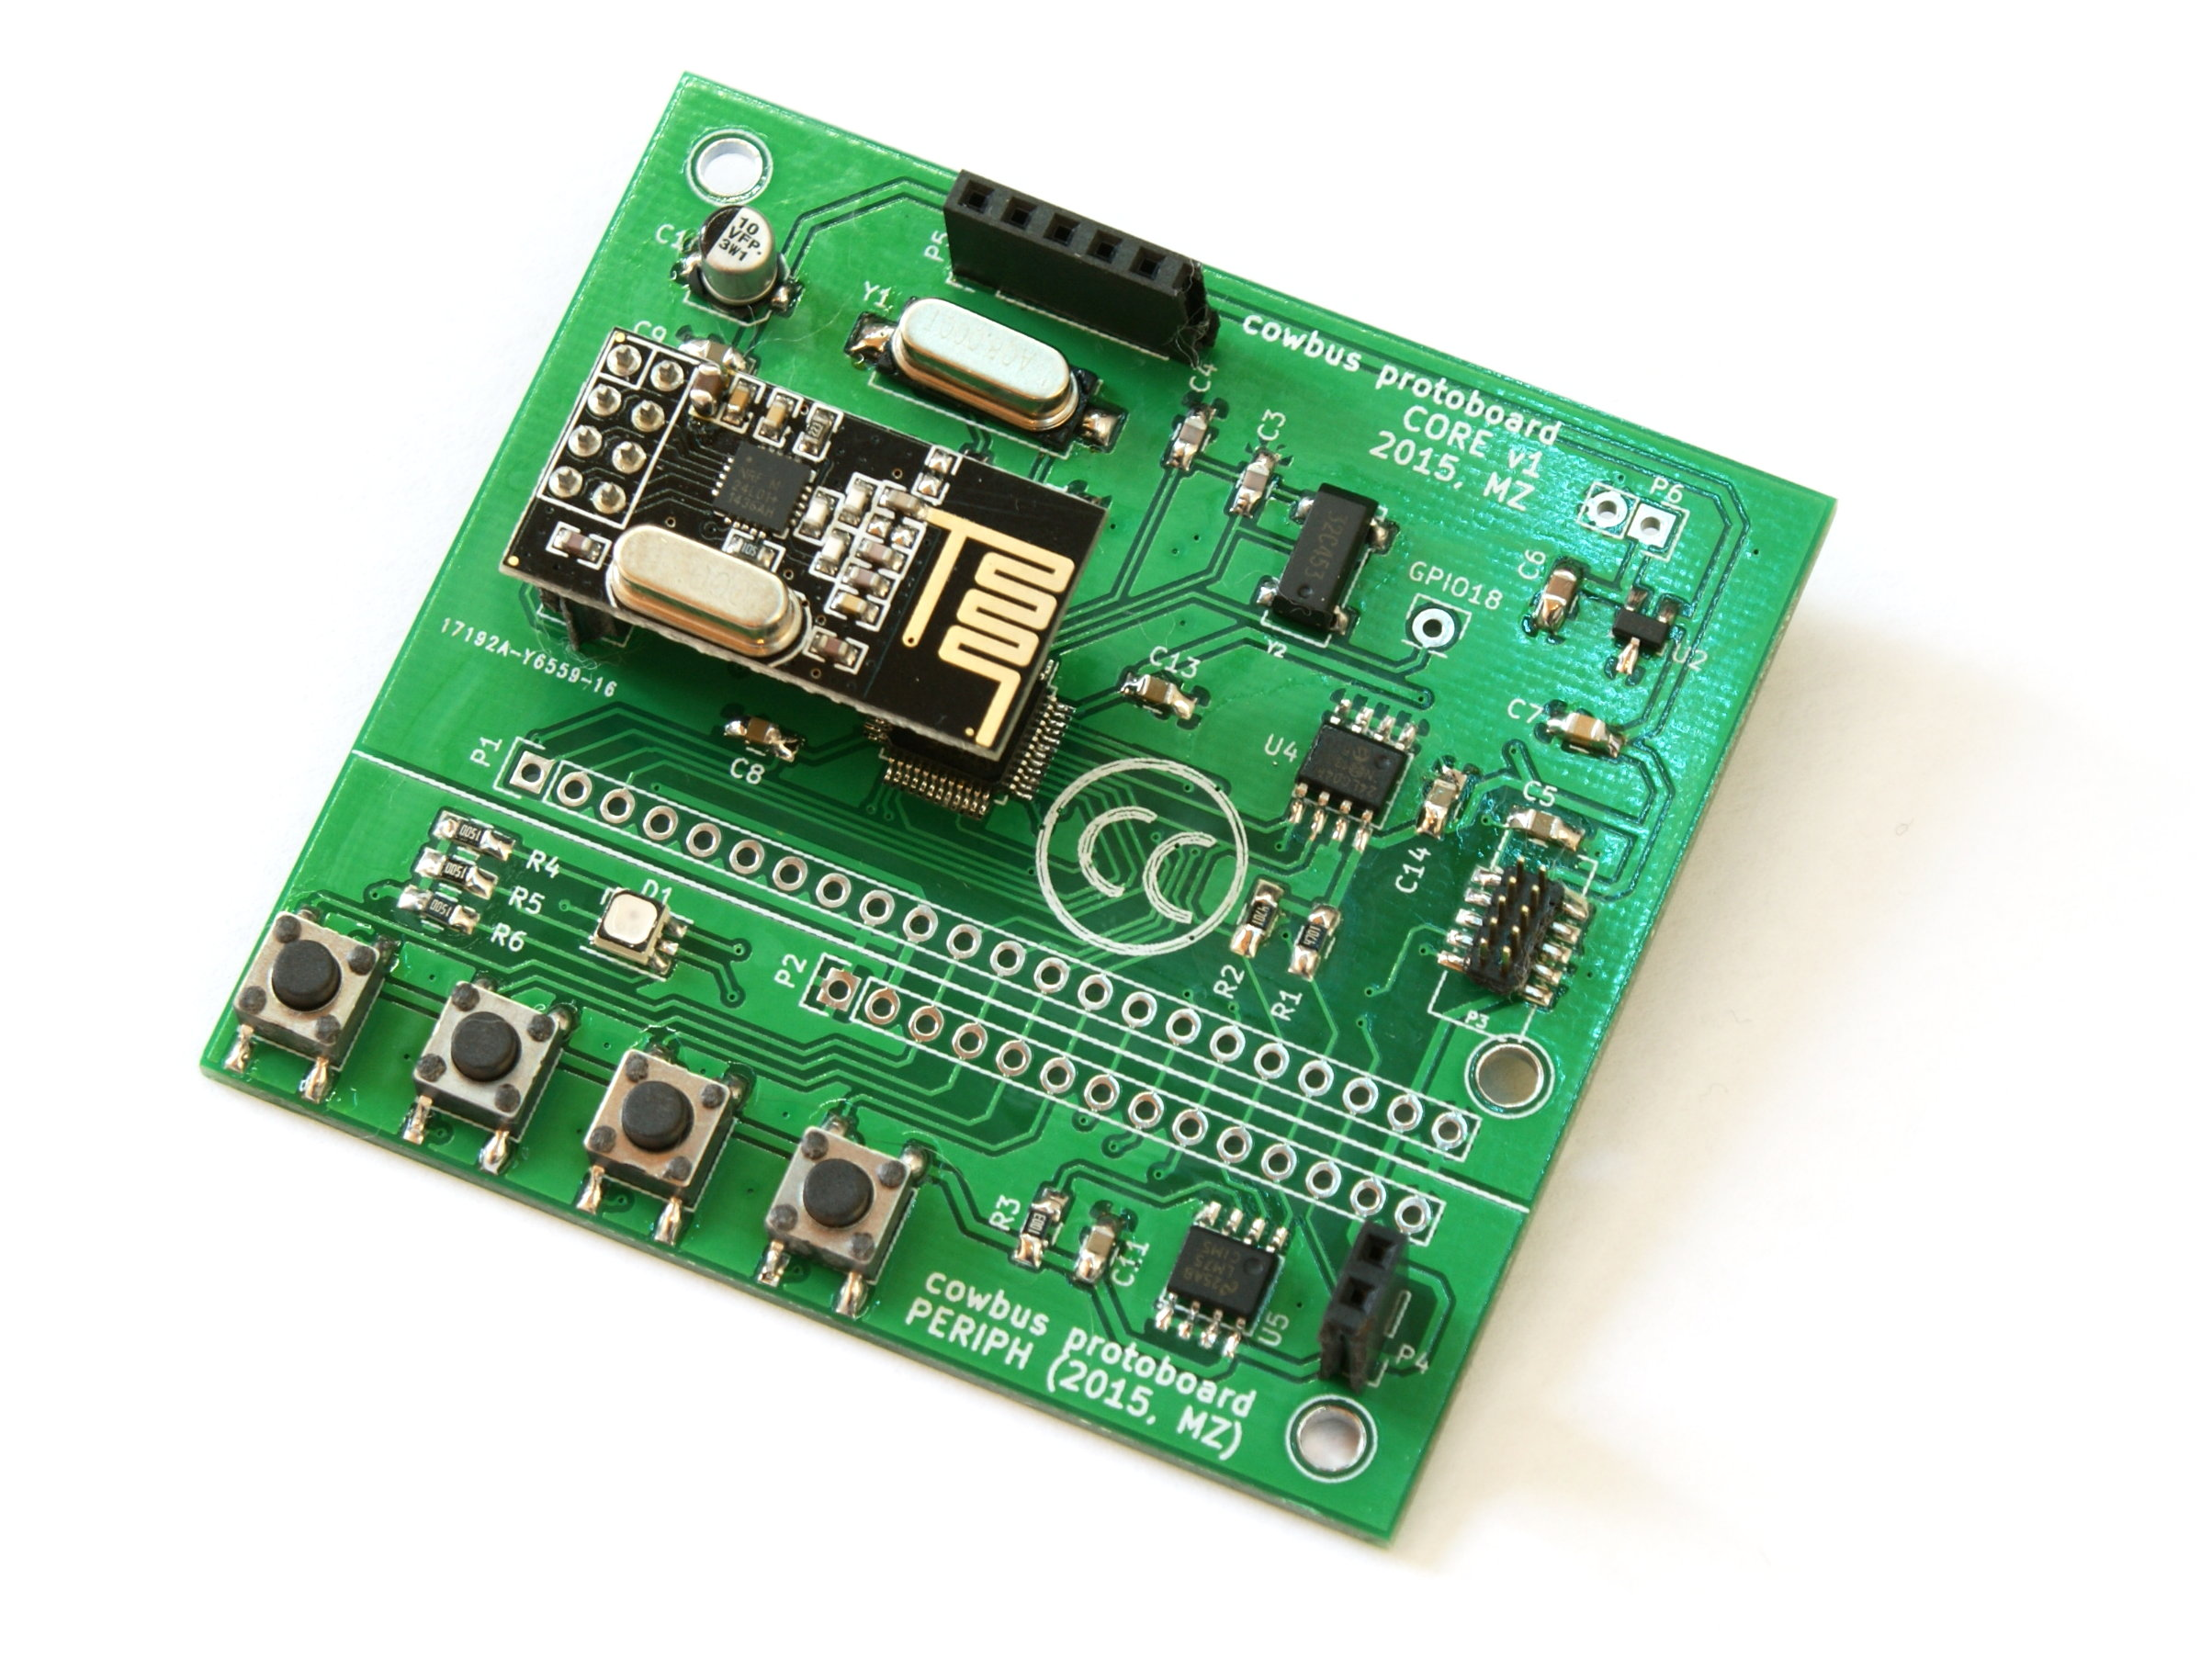
\includegraphics[width=.9\linewidth]{img/img-cowbus-proto.jpg}}
        	\uncover<3->{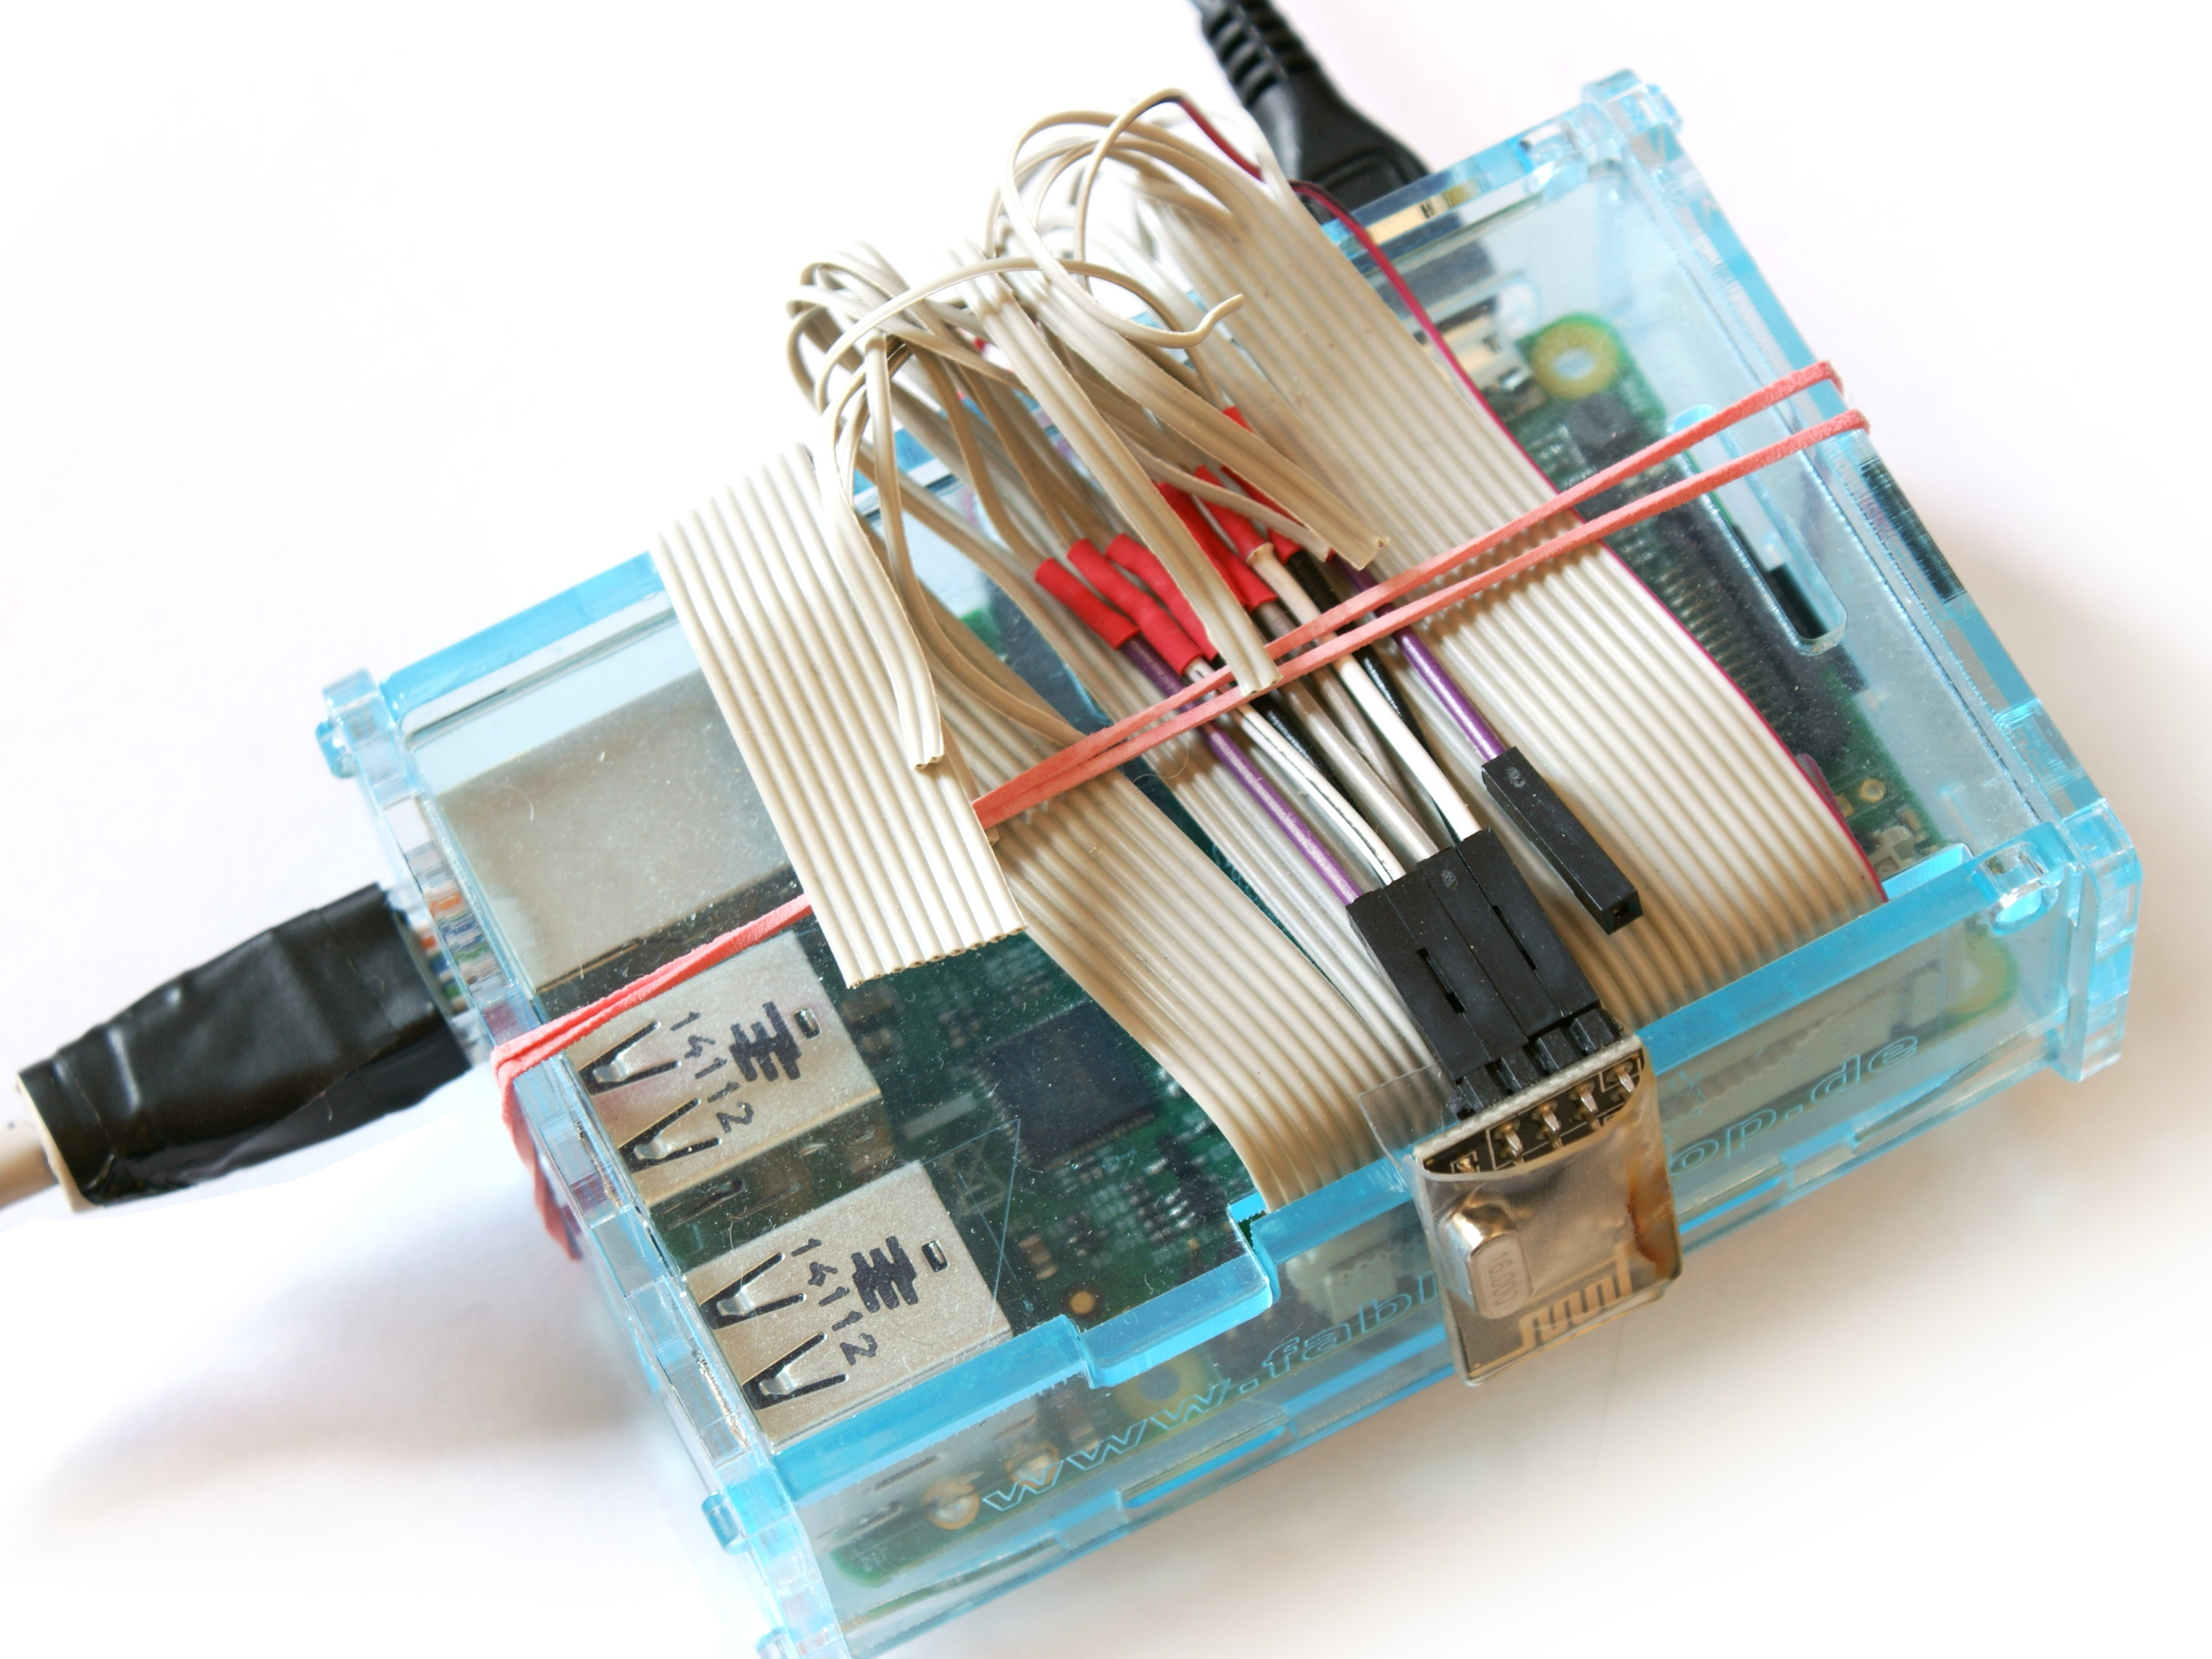
\includegraphics[width=.9\linewidth]{img/img-pi-rf.jpg}}
			\column{.6\textwidth}
		        \uncover<1->{
		       	Sensor:
        		\begin{itemize} \setlength{\itemsep}{\customitemsep}
                    \item cowbus-protoboard (OS: RIOT \cite{riot})
		            \item 4 Taster, Temperatursensor
		        \end{itemize}
		        \vspace*{0.75cm}
		        
		        Aktor:
		        \begin{itemize} \setlength{\itemsep}{\customitemsep}
                        \item cowbus-protoboard (OS: RIOT \cite{riot})
		            \item RGB-LED, Piezo-Summer
		        \end{itemize}
		        \vspace*{0.75cm}
		        }

				\uncover<3->{
		        Gateway:
		        \begin{itemize} \setlength{\itemsep}{\customitemsep}
		            \item Raspberry Pi B
		            \item Funkmodul per SPI angebunden
		        \end{itemize}
		        \vspace*{1cm}
		        }
		\end{columns}
\end{frame}

\begin{frame}
    \frametitle{Zusammenfassung \& Ausblick}

    \begin{itemize} \setlength{\itemsep}{\customitemsep}
		\item Open-Source-Hardware und -Software        
        \item einfache Konfiguration für \enquote{Jedermann}
        \item einfache Änderbarkeit
        \item Kommunikation in-band, keine Spezialhardware nötig
        \item[ ] \vspace*{0.5cm}
            \pause
        \item offene Fragen:
        	\begin{itemize}
        		\item komplexere Regeln?
		        \item Aggregation?
		        \item Bedeutung des Messwertes
		        \item Bedeutung der Aktion
        	\end{itemize}
    \end{itemize}
\end{frame}


\section{Vielen Dank für Ihre Aufmerksamkeit!}
\section{Q\&A}

\bibliography{2015-09-cowconfig}{}

%\begin{frame}[plain]
%    \center
%    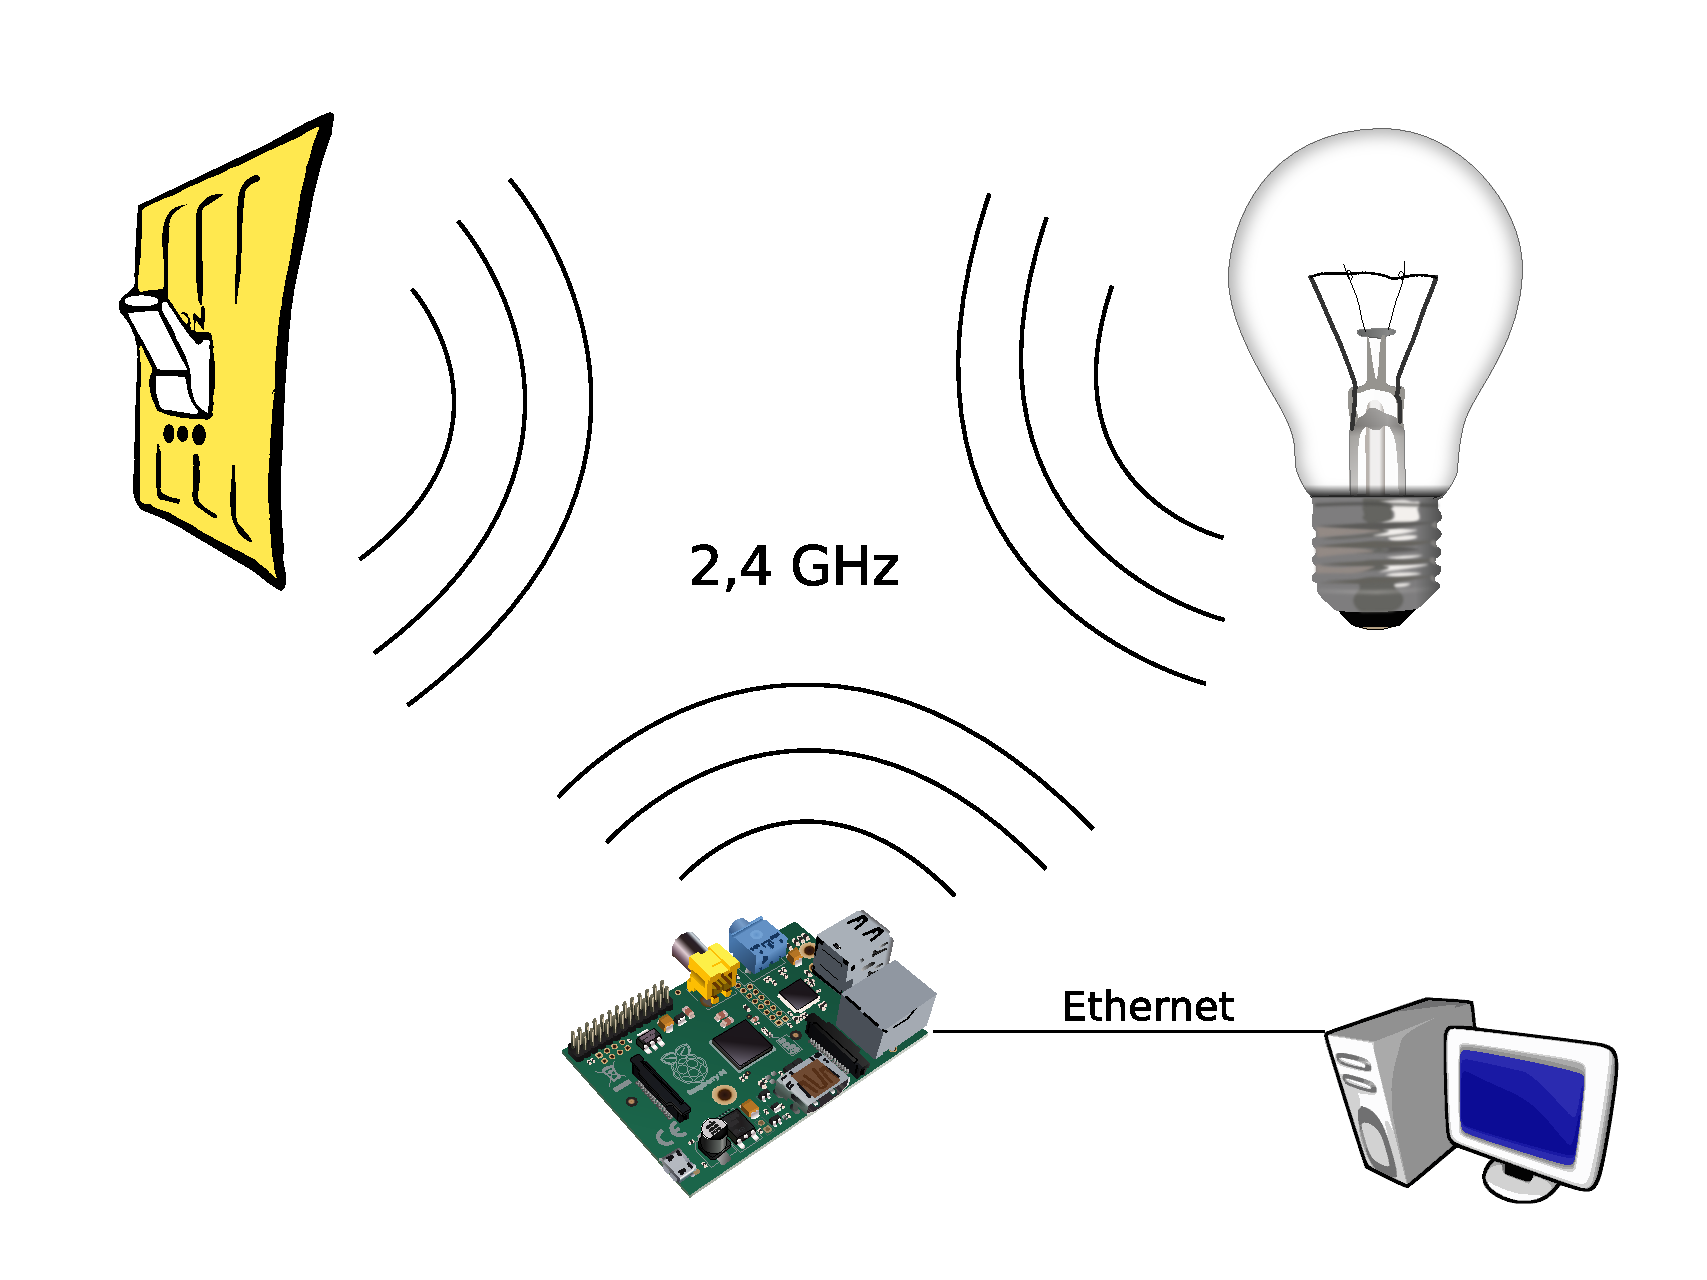
\includegraphics[scale=0.4]{img/system}
%\end{frame}


%\nocite*

\end{document}

